\chapter{Especificação e Modelação}

\section{Análise de Requisitos}

\subsection{Requisitos Funcionais}

\subsubsection{Requisitos Gerais de Anotação}

\begin{itemize}
    \item \textbf{RF1:} Gestão de diferentes formatos de dados (CSV, TXT, JSON, etc.)
    \item \textbf{RF2:} Sistema de organização hierárquica de datasets
    \item \textbf{RF3:} Exportação de dados anotados em múltiplos formatos
    \item \textbf{RF4:} Interface genérica para anotação de dados
    \item \textbf{RF5:} Suporte a múltiplos anotadores por dataset
    \item \textbf{RF6:} Distribuição automática de tarefas entre anotadores disponíveis
\end{itemize}

\subsubsection{Requisitos Específicos - Módulo Disentanglement}

\begin{itemize}
    \item \textbf{RF7:} Interface especializada para chat disentanglement
    \item \textbf{RF8:} Sistema de tagging para classificação de mensagens em threads
    \item \textbf{RF9:} Visualização sequencial dos turnos (mensagens)
    \item \textbf{RF10:} Calculo de métricas de anotação
\end{itemize}

\subsubsection{Gestão de Utilizadores}

\begin{itemize}
    \item \textbf{RF11:} Autenticação de utilizadores
    \item \textbf{RF12:} Definição de papéis (administrador/anotador)
    \item \textbf{RF13:} Controle de acesso baseado em permissões
\end{itemize}

\subsection{Requisitos Não Funcionais}

\subsubsection{Performance}

\begin{itemize}
    \item \textbf{RNF1:} Tempo de resposta adequado para operações interativas
    \item \textbf{RNF2:} Processamento eficiente para múltiplos utilizadores simultâneos
\end{itemize}

\subsubsection{Usabilidade}

\begin{itemize}
    \item \textbf{RNF3:} Interface responsiva e adaptável
    \item \textbf{RNF4:} Ferramenta interativa dando feedback visual claro das ações ao utilizador
    \item \textbf{RNF5:} Interface simples, minimalista e intuitiva
\end{itemize}

\subsubsection{Segurança}

\begin{itemize}
    \item \textbf{RNF6:} Backup automático de anotações
    \item \textbf{RNF7:} Logging de atividades críticas
\end{itemize}

\section{Modelação}

\subsection{Modelo de Dados}

O modelo de dados da plataforma é organizado em três componentes principais: gestão de utilizadores, gestão de dados e anotações. A estrutura completa, pode ser visualizada na Figura~\ref{fig:modelo-er}, que apresenta em detalhe as entidades e seus relacionamentos.

\subsubsection{Componentes Principais}

\paragraph{Gestão de Utilizadores}
O sistema mantém informações básicas dos utilizadores, incluindo credenciais e roles (administrador/anotador). Cada utilizador pode ter acesso a diferentes módulos de anotação, dependendo das permissões atribuídas.

\paragraph{Gestão de Dados}
Para o módulo de disentanglement, os dados são organizados em chatrooms, onde cada chatroom contém uma sequência de turnos (mensagens). Cada turno possui atributos como timestamp, autor e conteúdo. O conjunto total de chatrooms forma a base de dados a ser anotada. A ferramenta permite que diferentes módulos possam trabalhar com diversos formatos de dados (CSV, TXT, JSON, etc.).

\paragraph{Anotações}
As anotações são armazenadas independentemente dos dados originais, mantendo referências para a chatroom, turno, utilizador e timestamp. No contexto do disentanglement, cada anotação associa turnos a threads específicas, permitindo a reconstrução das conversas paralelas.

\subsubsection{Fluxo de Dados}

O fluxo de dados na plataforma segue o seguinte padrão:
\begin{enumerate}
    \item Importação de dados através da interface administrativa
    \item Distribuição automática de tarefas aos anotadores
    \item Processo de anotação no módulo específico
    \item Armazenamento contínuo das anotações via backend
    \item Cálculo de métricas e análise das anotações
\end{enumerate}

\subsubsection{Armazenamento}

A solução proposta contempla:
\begin{itemize}
    \item Sistema de arquivos estruturado para gestão de diferentes formatos de dados
    \item Base de dados para gestão de utilizadores e estado da aplicação
    \item Sistema de cache para otimização de performance
    \item Armazenamento independente de anotações para facilitar análise e processamento
\end{itemize}

Esta estrutura visa suportar diferentes tipos de dados e formatos, mantendo a flexibilidade necessária para implementação de novos módulos de anotação.

\section{Protótipos de Interface}

\subsection{Mapa de Navegação}

A estrutura de navegação da plataforma está idealizada para adaptar-se aos diferentes perfis de utilizador. O sistema prevê um portal de login onde após autenticação, os utilizadores terão acesso a um dashboard principal, que funcionará como ponto central de acesso às diversas funcionalidades da plataforma. A estrutura completa do mapa de navegação pode ser visualizada na Figura~\ref{fig:mapa-navegacao}, que foi modificada para ocupar uma página inteira em landscape.

A ferramenta de anotação será estruturada de forma modular, onde o dashboard principal permitirá acesso aos vários módulos disponíveis. Numa primeira fase, o módulo de disentanglement será o unico modulo desta arquitetura modular, no entanto o objetico da ferramenta de anotação será de acomodar mais módulos no futuro.

\subsection{Principais Interfaces}

\subsubsection{Portal de Entrada}
O acesso à plataforma é controlado através de um portal de autenticação minimalista. Esta decisão de design visa garantir a integridade dos dados e a atribuição correta das tarefas de anotação, sendo o login obrigatório para qualquer interação com os dados do sistema.

\subsubsection{Dashboard Principal}
Após autenticação, o utilizador acede a um dashboard que apresenta uma visão geral da plataforma. Este componente central adapta-se dinamicamente ao perfil do utilizador (administrador ou anotador), apresentando as funcionalidades relevantes e o estado atual das tarefas atribuídas.

\subsubsection{Módulo de Disentanglement}
O primeiro módulo implementado na plataforma foca-se na tarefa de disentanglement de chat, apresentando duas visões distintas:

\paragraph{Visão do Anotador}
Para os anotadores, a interface apresenta:
\begin{itemize}
    \item Lista das chatrooms atribuídas automaticamente pelo sistema
    \item Interface de anotação com visualização sequencial das mensagens
    \item Sistema intuitivo de tagging para classificação de threads
    \item Indicadores de progresso da tarefa
    \item Mecanismos de validação em tempo real
\end{itemize}

\paragraph{Visão do Administrador}
Os administradores têm acesso a funcionalidades adicionais:
\begin{itemize}
    \item Gestão completa dos datasets
    \item Monitorização do progresso dos anotadores
    \item Visualização de métricas e estatísticas
    \item Configuração da distribuição automática de tarefas
\end{itemize}

\subsubsection{Interface de Anotação}
O componente central do módulo de disentanglement é a interface de anotação, que foi projetada para maximizar a eficiência do processo de anotação. Cada chatroom é apresentada como uma sequência temporal de mensagens, onde o anotador pode facilmente:
\begin{itemize}
    \item Visualizar o contexto completo da conversa
    \item Criar e atribuir tags de thread às mensagens
    \item Acompanhar o progresso da anotação em tempo real
    \item Navegar eficientemente entre diferentes chatrooms
\end{itemize}

O sistema mantém um salvamento automático do progresso, permitindo que os anotadores retomem seu trabalho de forma seamless em qualquer momento.


\begin{figure}[p]
    \centering
    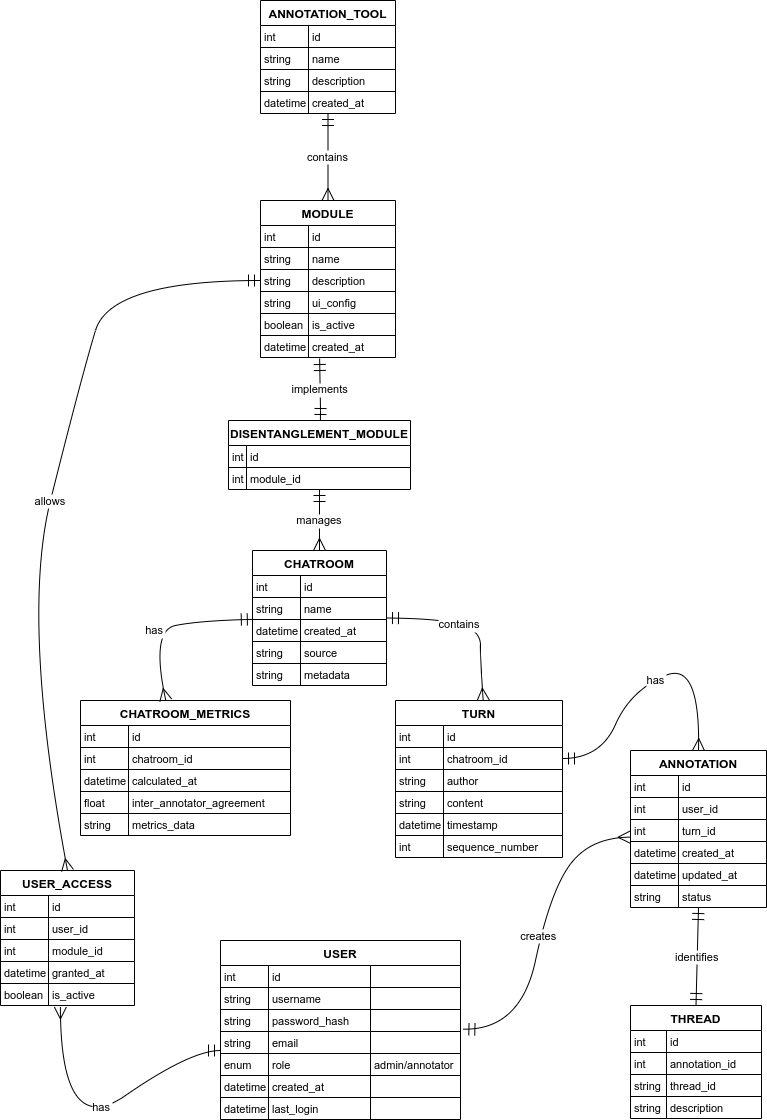
\includegraphics[width=0.95\textwidth,height=0.95\textheight,keepaspectratio]{images/Modelo_Entidade-Relacao.drawio.png}
    \caption{Modelo de Entidade-Relação do Sistema}
    \label{fig:modelo-er}
\end{figure}

\begin{landscape}
    \begin{figure}[p]
        \centering
        \makebox[\textwidth][c]{%
            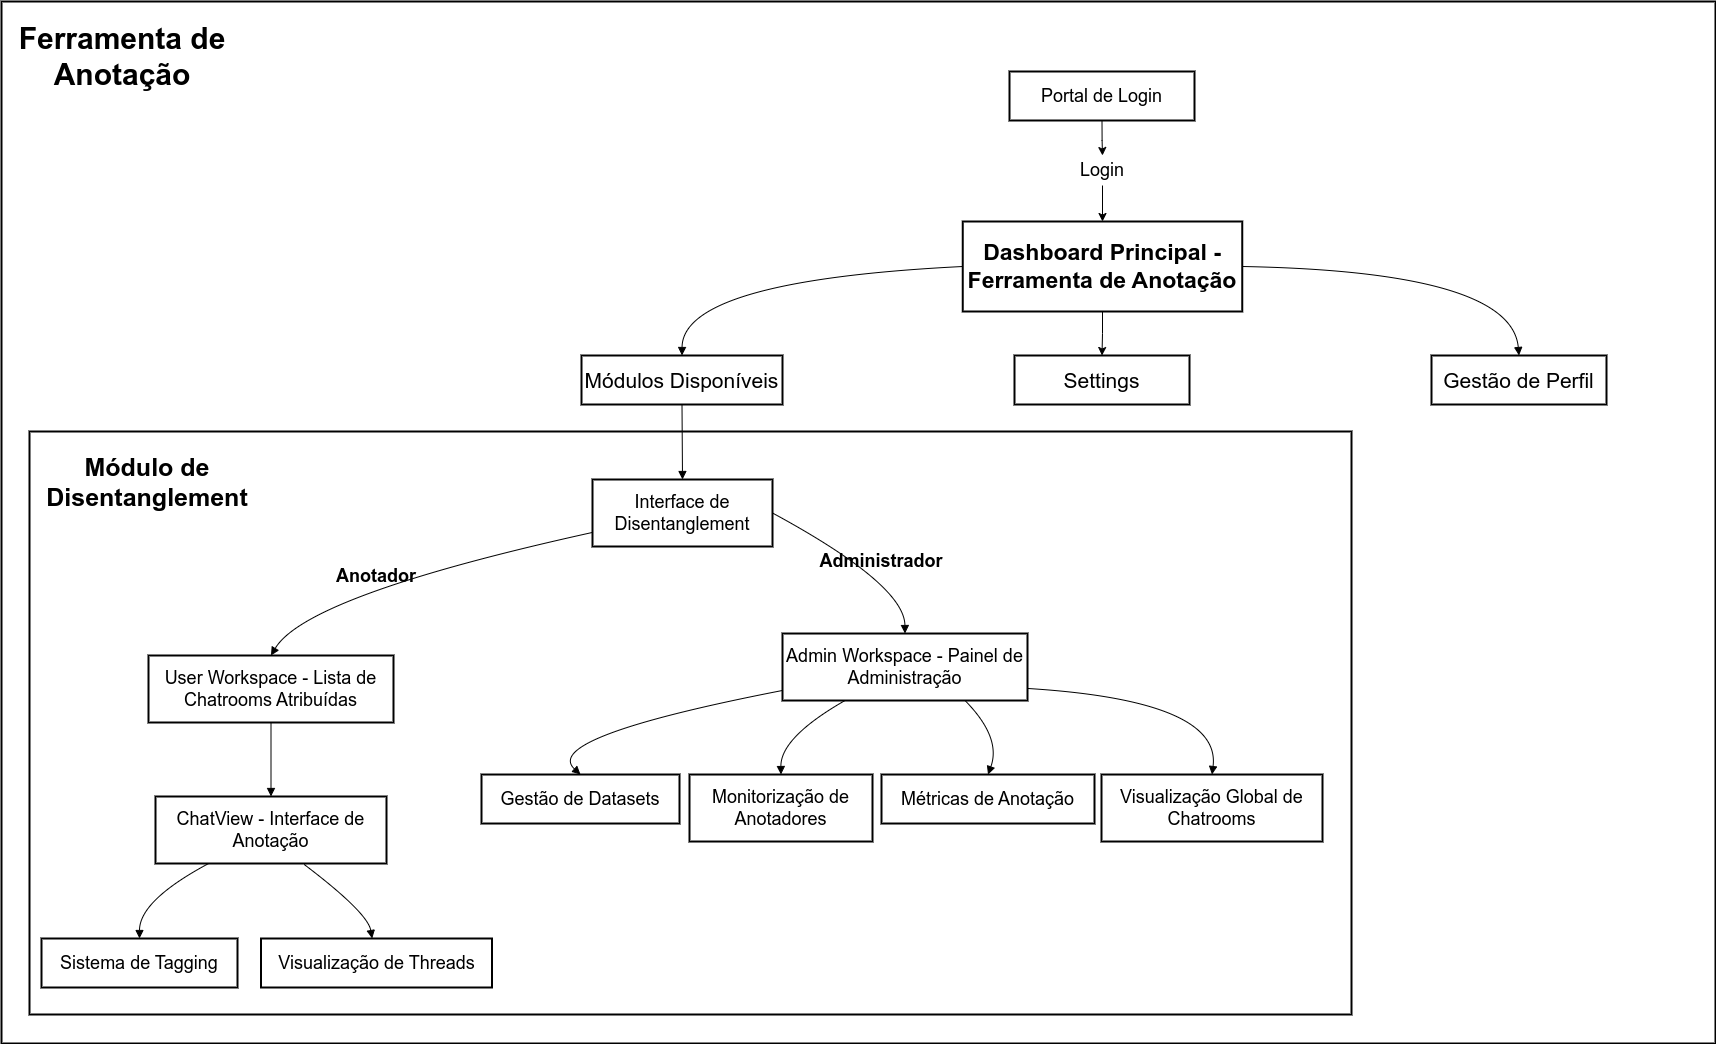
\includegraphics[width=0.8\paperheight, angle=0, keepaspectratio]{images/mapaDeNavegacaoSistema.drawio.png}
        }
        \caption{Mapa de Navegação do Sistema}
        \label{fig:mapa-navegacao}
    \end{figure}
\end{landscape}